Nguồn: \href{https://www.tiasang.com.vn/-khoa-hoc-cong-nghe/Anh-Dieu-12410}{Báo Tia Sáng}
\begin{figure}
\centering
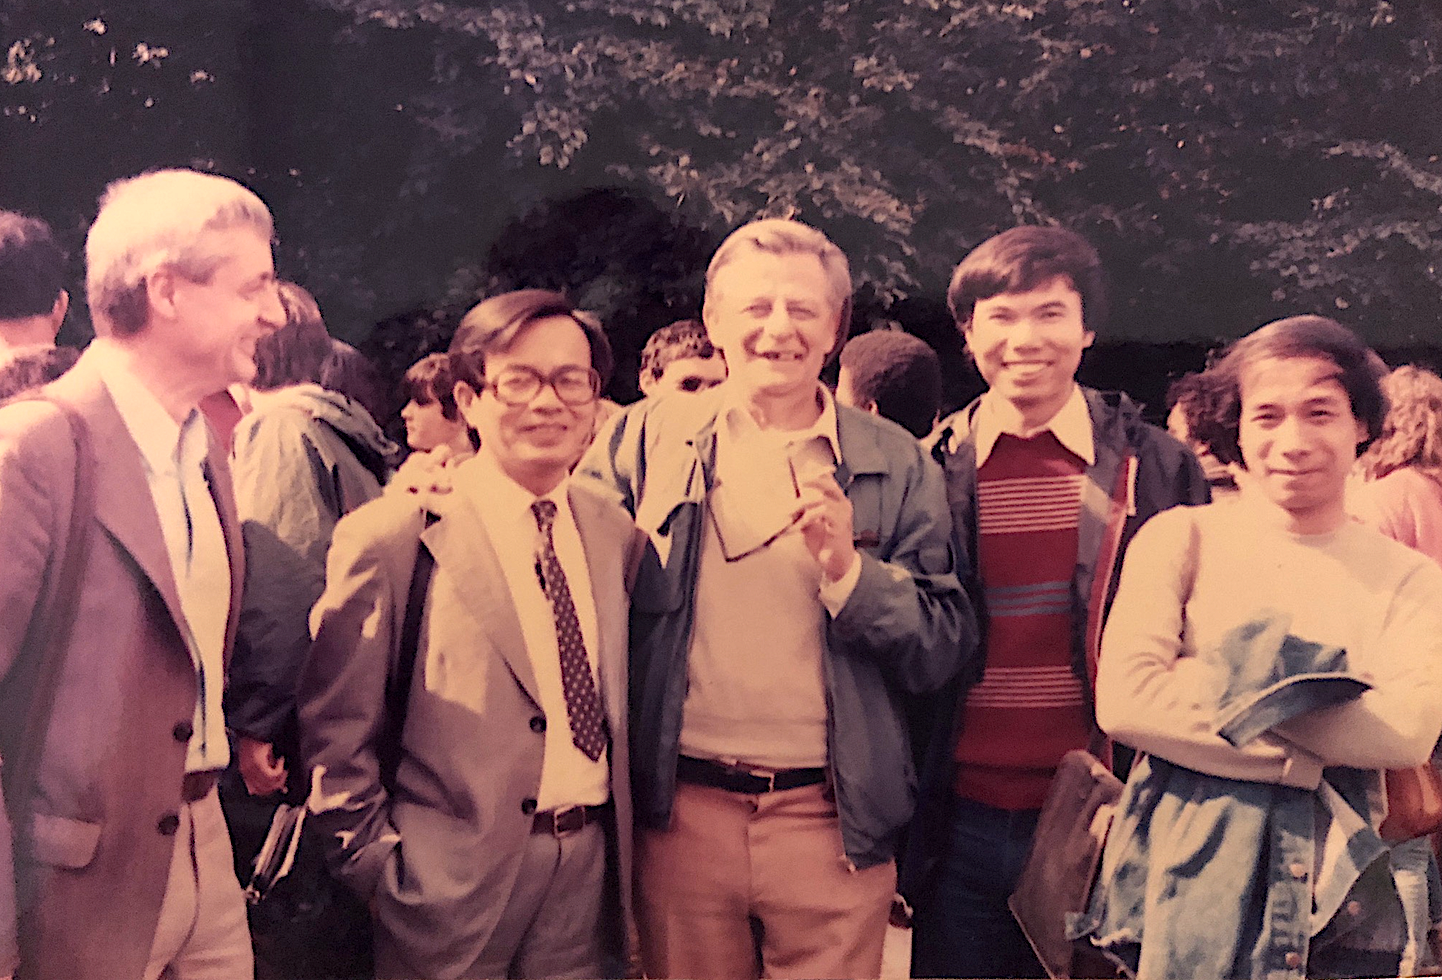
\includegraphics[scale=0.3]{Photos/Alain}
\caption{Từ trái qua: Kỹ sư Alain Teisonnière, anh Diệu, giáo sư Henri van Regemortor, Đặng Văn Đức và Hồ Tú Bảo (hai cán bộ của Viện) tại hội chợ Báo Nhân Đạo (l’Humanité), Paris 1985. Nguồn: Hồ Tú Bảo. }
\end{figure}


Xin được gọi anh là một hào kiệt và người anh cả của tin học Việt Nam.


Đúng nửa thế kỷ trước chúng tôi là những cô bé cậu bé lớp chuyên toán của Trường Đại học Sư phạm Hà Nội, sơ tán ở làng Viên Nội bên bờ sông Đáy. Mỗi chiều muộn thứ bảy lại thấy một người đẹp trai đạp xe về Viên Nội thăm vợ là cán bộ đi học ở Khoa Toán mới sinh con. Mọi người bảo nhau đấy là nhà toán học Phan Đình Diệu, mới tốt nghiệp tiến sĩ khoa học ở Liên Xô về nước. Hồi ấy số tiến sĩ khoa học của cả nước chỉ đếm trên đầu ngón tay. Sáng chủ nhật thấy nhà toán học mang một chậu quần áo tã lót đi giặt, rồi gánh nước từ giếng làng về đổ bể như lũ học trò chúng tôi.

Câu chuyện tuổi thơ ấy bẵng đi chục năm khi tôi đang học dở ngành toán thì đi lính,có những ngày Quảng Trị hè 1972, bị thương và về học tiếp chương trình đại học ngành toán ứng dụng. Ra trường, người bạn thân đang làm ở Viện Khoa học Tính toán và Điều khiển của Viện Khoa học Việt Nam, nay là Viện Hàn lâm KH\&CN Việt Nam, rủ tôi xin về Viện và dẫn đến gặp Viện trưởng. Gặp lại anh, người gánh nước cùng chúng tôi năm xưa.

Xem tên các môn học rất mới của Khoa Toán-Lý Bách Khoa hồi đó, hỏi về luận án tốt nghiệp và khen học tốt, anh đồng ý nhận tôi về Viện. Ít ngày sau tôi thành một “viện sĩ” như tụi tôi vẫn đùa (cũng lúc ấy có chuyện một cô gái tốt nghiệp ở Đức về, mang lá thư của người bác đang làm Bộ trưởng đến đề nghị anh Diệu nhận về Viện, anh đã dứt khoát từ chối).

Có một thời gian dài là “quân anh Diệu”, nhớ và nghĩ về anh tôi thấy rõ mấy điều sau.

1. Sự dấn thân của anh Diệu vào lĩnh vực tin học (còn được gọi với các tên công nghệ thông tin hay khoa học máy tính). Theo quan sát của tôi, mỗi lĩnh vực khoa học ở mỗi quốc gia có những người vượt trội trong quãng thời gian một vài chục năm. Đó là những người có tài năng xuất chúng và có sự phấn đấu bền bỉ. Trong toán học Việt Nam đó là các giáo sư Lê Văn Thiêm, Hoàng Tuỵ, rồi nhiều năm sau là Ngô Bảo Châu… Trong tin học tôi nghĩ đấy là anh Diệu.

Trong những năm đầu nghiên cứu toán anh Diệu đã đạt những kết quả rất xuất sắc, và tôi tin anh sẽ làm được rất nhiều nữa nếu tiếp tục con đường này. Nhưng trong những năm tháng chiến tranh ấy chúng ta đã có những chiếc máy tính lớn Minsk 22 của Liên Xô, ODRA 1304 của Ba Lan… và cần dùng chúng cho các nhiệm vụ quốc gia. Được giao trọng trách xây dựng và phát triển ngành tin học, anh Diệu đã dành hầu hết thời gian để tự học và nghiên cứu về tin học, một lĩnh vực mới rất đa dạng và phong phú.

Khác với toán học nơi người làm toán thường nghiên cứu độc lập và có thể chỉ cần bút và giấy, tin học vừa có phần lý thuyết luôn thay đổi rất nhanh, vừa gắn với công nghiệp máy tính (phần cứng), vừa gắn với phát triển các thuật toán và chương trình (phần mềm), và vừa gắn với các hệ thống ứng dụng (ở ta hồi đó là những nhiệm vụ tính toán khoa học trong khí tượng và địa chất…). Dân tin học cũng thường không làm việc độc lập, mà phải liên kết trong cácnhóm. Người phụ trách tin học bắt buộc phải đọc và học nhiều kiến thức khác nhau, thường xuyên thay đổi. Phải có niềm ham mê đặc biệt và một trí lực phi thường mới có thể đọc và hiểu được nhiều thứ như vậy, để có thể dẫn dắt một tập thể, để có thể chia sẻ và thuyết phục một cộng đồng. Và anh Diệu đã làm như vậy.

Kiên định với những quan điểm riêng là điều luôn nhất quán ở anh Diệu.

Trong quỹ thời gian hạn chế, anh Diệu vẫn làm nghiên cứu về toán. Anh viết bài về mật mã, về lập luận xác suất… Anh viết sách về lý thuyết automat và thuật toán, sách về logic toán. Hơn mười năm trước tôi có dịp mời anh thăm Viện Khoa học và Tiên tiến Nhật Bản và trao đổi với giáo sư Ono, chuyên gia hàng đầu về logic toán của Nhật. Câu chuyện của hai vị giáo sư tuổi bảy mươi sôi nổi, sâu sắc, đầy thú vị và uyên bác.

Với anh Diệu, tôi hiểu việc gác lại con đường làm toán để dành tâm sức cho sự phát triển nền tin học nước nhà từ thuở sung sức của đời làm khoa học là một lựa chọn đúng đắn. Anh làm được nhiều hơn cho cộng đồng và đất nước.

2. Tầm nhìn sâu rộng của anh Diệu và những đóng góp của anh về chính sách phát triển tin học quốc gia. Tiêu biểu nhất là ba lần anh Diệu chủ trì việc xây dựng chương trình quốc gia về công nghệ thông tin.

Ngay từ khi mới đi làm tôi đã có dịp xem tập tài liệu rất dầy do anh Diệu và anh Trần Lưu Chương (khi đó phụ trách Cục máy tính của Bộ Khoa học và Công nghệ) viết xong vào năm 1976. Tài liệu này trình bày bức tranh tổng thể về tin học trên toàn thế giới và đề xuất kế hoạch phát triển ngành tin học Việt Nam. Vào năm 1976 sinh viên tụi tôi vẫn lập trình trên các băng từ đục lỗ, thì một chương trình chi tiết như vậy cho thấy người viết đã có tầm nhìn rất xa và cái nhìn đã rõ khi vạch con đường của tin học Việt Nam.

Nhưng đề xuất năm 1976 này đã chưa được phê duyệt. Trong các năm 1981 và 1982, dưới sự chỉ đạo tâm huyết của anh Diệu, nhóm các nhà khoa học trẻ của Viện Khoa học Tính toán và Điều khiển đã thiết kế và chế tạo chiếc máy vi tính mẫu đầu tiên của Việt Nam, như một trong những chiếc máy vi tính được chế tạo sớm ở châu Á. Vào năm 1984 khi Việt Nam vẫn đang bị cấm vận, anh Diệu lại chủ trì đưa ra một bản mới của chương trình. Vẫn thường được xem là những chiếc máy và chương trình "đẻ non" khi xã hội chưa sẵn sàng, cácbước đi đầu này đã dẫn đến những bước đi tiếp theo.

Không nao núng với hai lần chưa thành công trước đó, anh Diệu- người chấp bút không mỏi mệt- đã có một bản dự thảo của chương trình được phê duyệt vào mùa hè 1994 theo Nghị định 49/CP, và từ đó một chương trình quốc gia về công nghệ thông tin đã được tiến hành.

Năm 1984 khi tôi học xong DEA (chương trình thạc sĩ ở Pháp) về xử lý ảnh và chuẩn bị tiếp tục làm luận án theo hướng này. Trong một bức thư gửi từ Việt Nam qua anh Diệu viết “nếu có thể Bảo nên chuyển qua làm về trí tuệ nhân tạo vì đấy là tương lai của tin học”. Theo lời anh tôi đã chuyển hướng, dù mất công hơn vì chưa biết gì về chuyện này. Bây giờ sau hơn ba chục năm, trí tuệ nhân tạo ngày càng có vai trò thiết yếu trong thời chuyển đổi số, càng thấy tầm nhìn của anh.

3. Những ý kiến đóng góp của anh Diệu về xây dựng đất nước. Là người luôn trăn trở, suy nghĩ về những vấn đề của phát triển đất nước, anh Diệu đã luôn thẳng thắn nêu những chính kiến của mình.

Đấy là những ý kiến anh phát biểu tại Quốc hội, tại Mặt trận Tổ quốc Việt Nam khi anh là thành viên của các tổ chức này. Đấy là các ý kiến khi anh gặp các lãnh đạo cấp cao của Đảng cộng sản và nhà nước. Đấy là các bài viết đầy tâm huyết và trăn trở về con đường phát triển đất nước. Kiên định với những quan điểm riêng là điều luôn nhất quán ở anh Diệu.

4. Mối quan hệ chân tình của anh Diệu với bạn bè và đồng nghiệp. Trong quan sát của tôi, bạn bè nước ngoài đến làm việc ở Việt Nam đều tỏ rõ sự quý trọng với anh. Đó là các nhà triết học của Viện Hàn lâm Nga khi đến Việt Nam đã duy nhất mời anh Diệu viết với họ về triết học trong khoa học, là giáo sư Henri van Regemorter và kỹ sư Alain Teissonnière từ Pháp khi giúp ta phát triển tin học, là vợ chồng nhà toán học Đức Klaus và Angela Krickerberg sang dạy về dịch tễ học, là giáo sư Judy Ladinsky giúp ta xây dựng hợp tác khoa học Mỹ-Việt từ khi đất nước bị cấm vận… Anh Diệu cũng được các anh chị Việt kiều rất quý trọng, và nhiều người đã về giúp Việt Nam theo lời mời của anh. Tôi thấy hầu hết những người làm việc cùng đều quý trọng anh. Anh Diệu không lấy lòng người khác, mà bằng trí tuệ và nhân cách, bằng công việc chung, bằng sự chân tình, anh thu phục lòng người. Với những người trẻ hơn như tụi tôi, anh còn có nhiều chia sẻ, chỉ dẫn ân cần.

Tôi tự hỏi nếu chỉ dùng một vài từ để nói về anh Diệu, sẽ là gì?

Hồi nhỏ tôi mê mẩn “Lá cờ thêu sáu chữ vàng” của nhà văn Nguyễn Huy Tưởng viết về Trần Quốc Toản với hình ảnh của “sáu trăm gã hào kiệt”, và nhớ đến cả nước đã trân trọng gọi Đại tướng Võ Nguyên Giáp là “người anh cả của quân đội nhân dân Việt Nam”. Với anh Diệu, xin được gọi anh là một hào kiệt và người anh cả của tin học Việt Nam.

Năm 1954 sau ngày hoà bình lập lại ở miền Bắc, vừa học xong phổ thông ở quê Hà Tĩnh, như nhiều chàng trai trẻ miền Trung đầy nghị lực, anh Diệu đi bộ ra Hà Nội thi vào trường Đại học Khoa học, rồi theo học trường Đại học Sư phạm Hà Nội. Tốt nghiệp thủ khoa ngành Toán, anh tham gia giảng dạy ở đây 5 năm cho đến 1962 được cử đi làm nghiên cứu sinh về Toán ở trường Đại học Tổng hợp Moscow. Lĩnh vực nghiên cứu lúc đó của anh Diệu là toán học kiến thiết. Nói nôm na, đây là lĩnh vực nhằm không những chỉ ra các sự “tồn tại” trong toán học mà còn chỉ ra liệu “ta có thể xây dựng” được chúng với các thuật toán. Luận án tiến sĩ khoa học của anh Diệu dựa trên sáu bài báo anh đăng trên tạp chí “Doklady Akademii Nauk” nổi tiếng ở Nga, sau được in trong cuốn sách “Một số câu hỏi về giải tích hàm kiến thiết” ở Nga và ở Mỹ. Năm 1967 sau khi bảo vệ luận án tiến sĩ khoa học, anh Diệu về nước tham gia xây dựng Phòng Toán học Tính toán của Ủy ban Khoa học và Kỹ thuật Nhà nước, tiền thân của Viện Khoa học Tính toán và Điều khiển (cũng như các Phòng Toán học, Phòng Vật Lý... là tiền thân của Viện Toán học, Viện Vật lý... của Viện Khoa học Việt Nam).